\chapter{Ejercicios}
\newpage
\section{Guía 1}

\subsection{Ejercicio 1}
Escriba un programa que le haga ingresar un número entero entre 1 y 499 y que lo escriba en nomenclatura romana. Si el numero no es entero o no está entre 1 y 499, que vuelva a pedir un nuevo número.
\subsection{Ejercicio 2}
Escriba un programa que le haga ingresar el nombre de una serie, los capítulos que posee y los minutos que duran cada uno, y que devuelva los dias, las horas y minutos que demoraría en ver todos los capítulos de la serie. Ej: te demorarías 309 horas y 29250 minutos en ver One Piece.
\newpage

\section{Guía 2}
\subsection{Ejercicio 1}
Haga un script que al ingresar como parámetro un planeta del sistema solar(hacerlo directamente desde la terminal), te indique el diametro ecuatorial en kilometros.El script debe reconocer el planeta en 3 distintos formatos. Ej: Tierra,TIERRA,tierra
\subsection{Ejercicio 2}
Haga un script que al ingresar el número de dureza según la escala de Mohs de una roca, te indique la categoría de la roca(Blanda,Dura,etc)
\newpage
\section{Guía 3}
\subsection{Ejercicio 1}
Del siguiente sitio web: \\
\url{https://raw.githubusercontent.com/plotly/datasets/master/volcano_db.csv} \\
Guarde en un archivo nuevo todas las lineas en donde es mencionado Chile.
\subsection{Ejercicio 2}
Del siguiente sitio web: \\
\url{https://raw.githubusercontent.com/plotly/datasets/master/volcano_db.csv}
Ordene el documento alfabéticamente según la columna 3(Country)(Pista: ver el manual de sort). 
\begin{figure}
	
\end{figure}
\newpage
\section{Guía 4}
\subsection{Ejercicio 1}
Mediante la siguiente matriz:\\
A=[2 -5 9 3;1 -2 4 5; 2 -3 5 7];\\
obtenga la matriz escalonada sin ocupar ninguna función, solamente con operaciones matriciales. Puede comprobar su resultado ocupando rref(A)
\subsection{Ejercicio 2}
Mediante la siguiente matriz:\\
B = [1 -2 4; -5 2 0; 1 0 3]; \\
Calcule el determinante de B sin ocupar ninguna función,solamente con operaciones. Puede comprobar su resultado con det(B)\newpage
\section{Guía 5}
\subsection{Ejercicio 1}
El siguiente archivo contiene los casos diarios de covid19 en Chile desde el 2 de Marzo de 2020 hasta el 20 de Julio de 2021: \\
\url{https://raw.githubusercontent.com/alvillaca/Files-PNG/main/casosdiarios.txt}\\
Cree un gráfico de los casos diarios respecto a la fecha y el polinomio de grado 7 correspondiente. El gráfico debería verse así:
\begin{figure}[h]
	\centering
	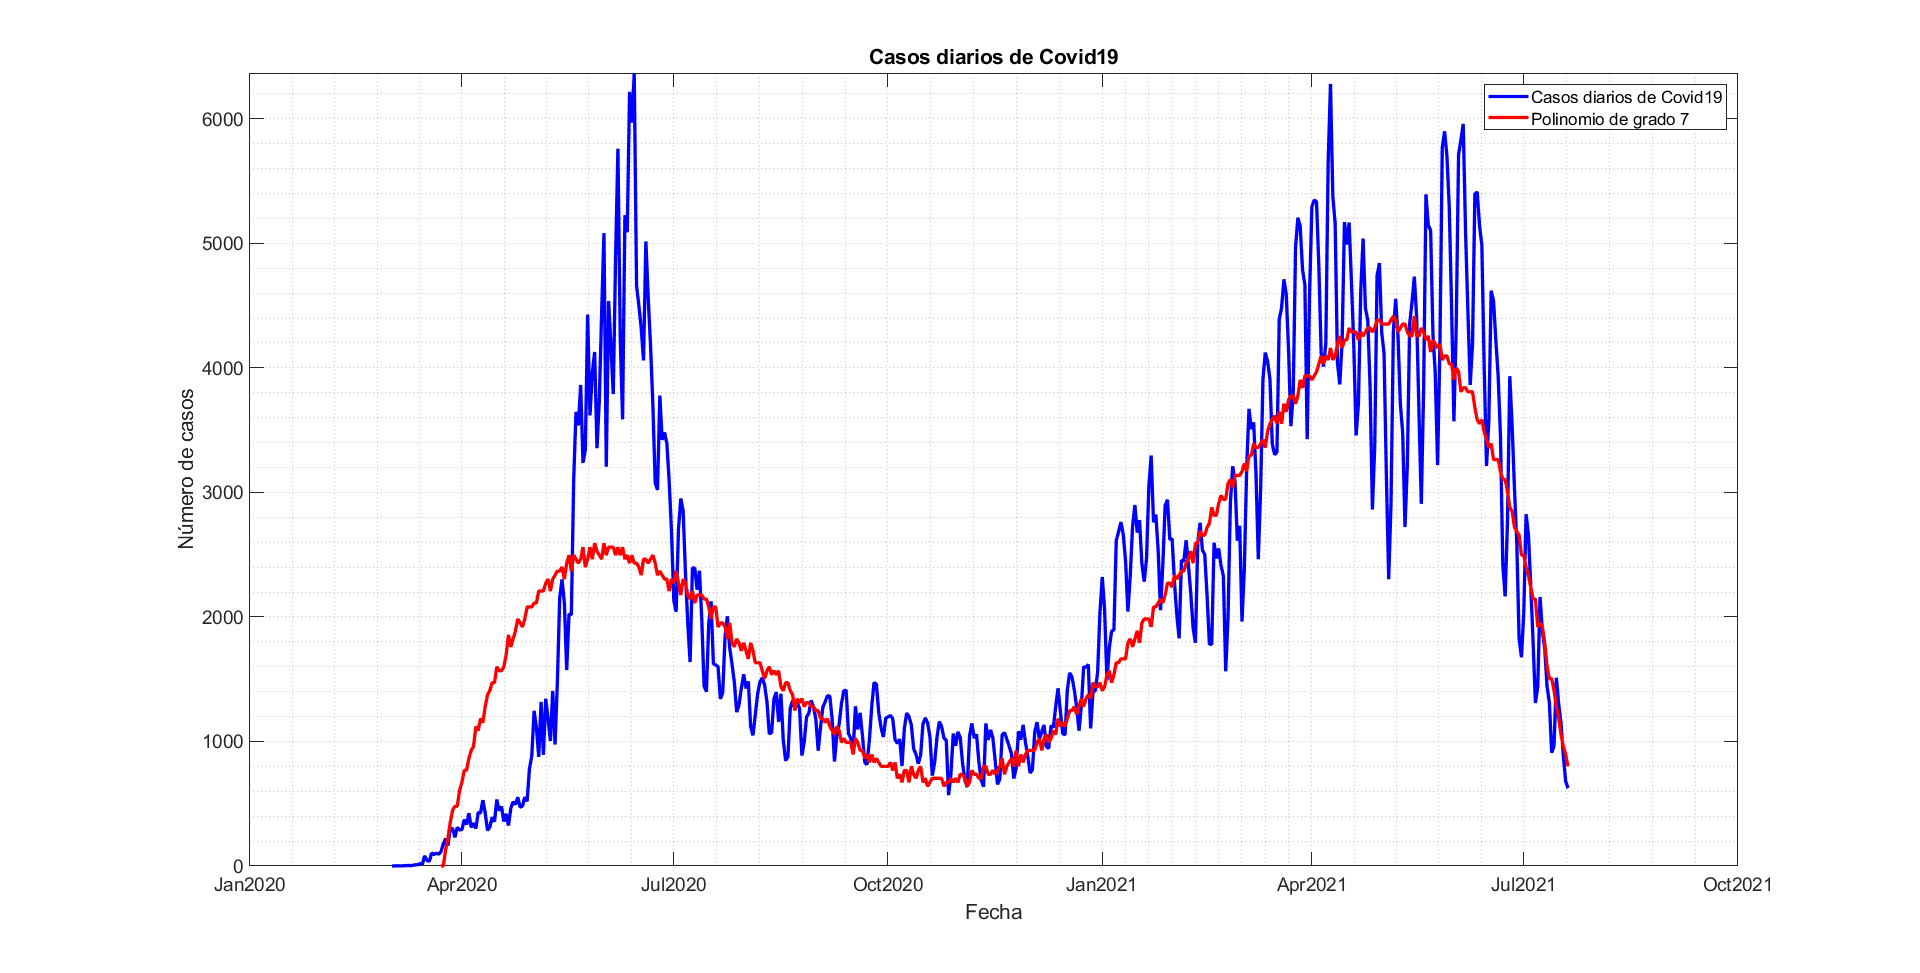
\includegraphics[width=0.7\linewidth]{Matlab/covid}
	\caption{Casos Covid19 diarios en Chile}
	\label{fig:covid}
\end{figure}

\subsection{Ejercicio 2}
Al gráfico anterior, agreguele los principales estadísticos(Media,Mediana,1er Q y 3er Q.El gráfico debería verse así:\
\begin{figure}[h]
	\centering
	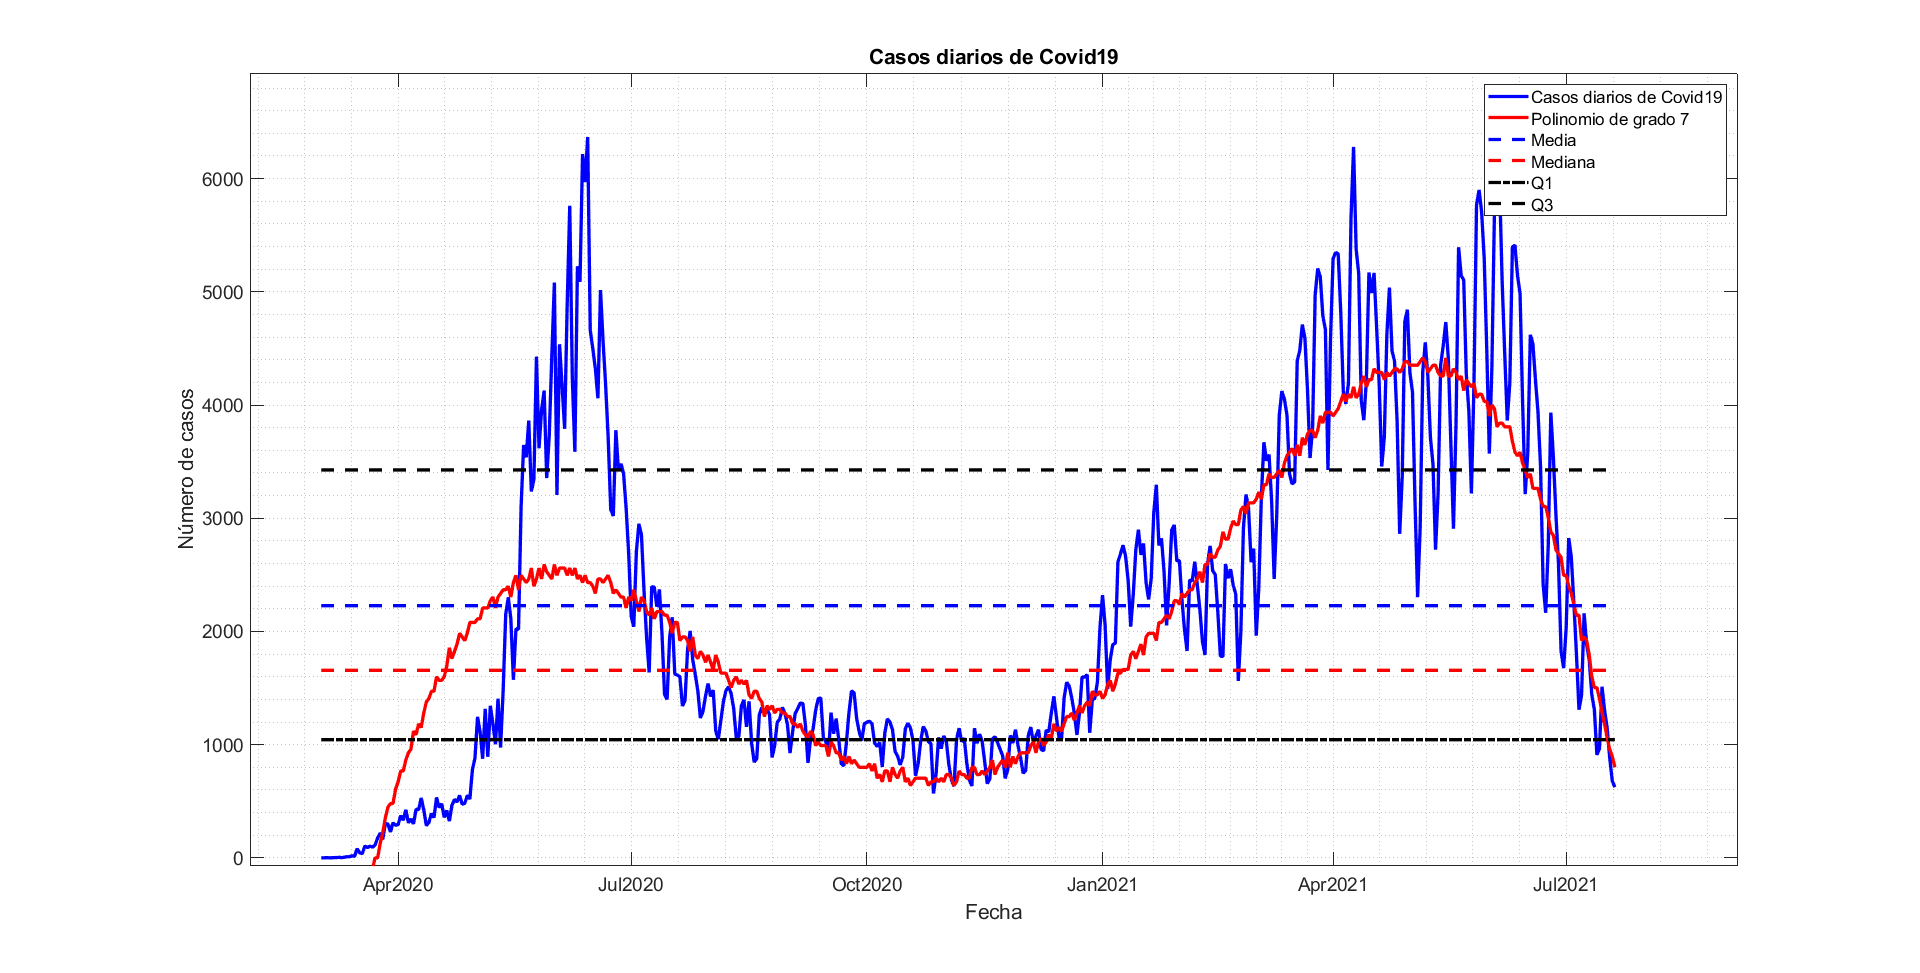
\includegraphics[width=0.7\linewidth]{Matlab/covid2}
	\caption{Casos covid19 diarios en Chile + Estadísticos}
	\label{fig:covid2}
\end{figure}
\newpage
\section{Guía 6}
\subsection{Ejercicio 1}
Defina una función que al ingresar un número natural, devuelva la secuencia de fibonacci con el número de terminos que ud indicó. Si el número ingresado no es natural, o no es un número,pedir un nuevo número y retornar a la función nuevamente. Ejemplo:
\begin{lstlisting}
	>> fibo(1.1)
	Ha ingresado un numero decimal,intente nuevamente
	Ingrese un numero natural: 
	12
	
	ans =
	
	0     1     1     2     3     5     8    13    21    34    55    89
	
	>> fibo('hola')
	No ha ingresado un numero,
	Ingrese un numero natural: 
	12
	
	ans =
	
	0     1     1     2     3     5     8    13    21    34    55    89
\end{lstlisting}
\subsection{Ejercicio 2}
Defina una función que al ingresar un vector, lo ordene de menor a mayor. Si lo ingresado no es un vector, pedir ingresar un vector y retornar a la función nuevamente. Ejemplo:
\begin{lstlisting}
ordenar([1,1;1,1])
No ha ingresado un vector, intente nuevamente: 
Ingrese un vector 
[10 4 2 5 3]
2     3     4     5    10
\end{lstlisting}\newpage
\section{Guía 7}
\subsection{Ejercicio 1}
Descargue la siguiente base de datos de covid19 en Chile:\\
https://raw.githubusercontent.com/alvillaca/Files-PNG/main/TotalesNacionales.csv\\
Cargue el archivo y organice en una estructura la fecha(debe dejarla en formato datetime), los casos nuevos con sintoma, los casos totales, los casos recuperados, los fallecidos y los casos activos(Pista: para cargar el archivo puede ocupar importdata).Finalmente, realice una figura de 5 subplots, con cada campo creado. 
\begin{figure}[h]
	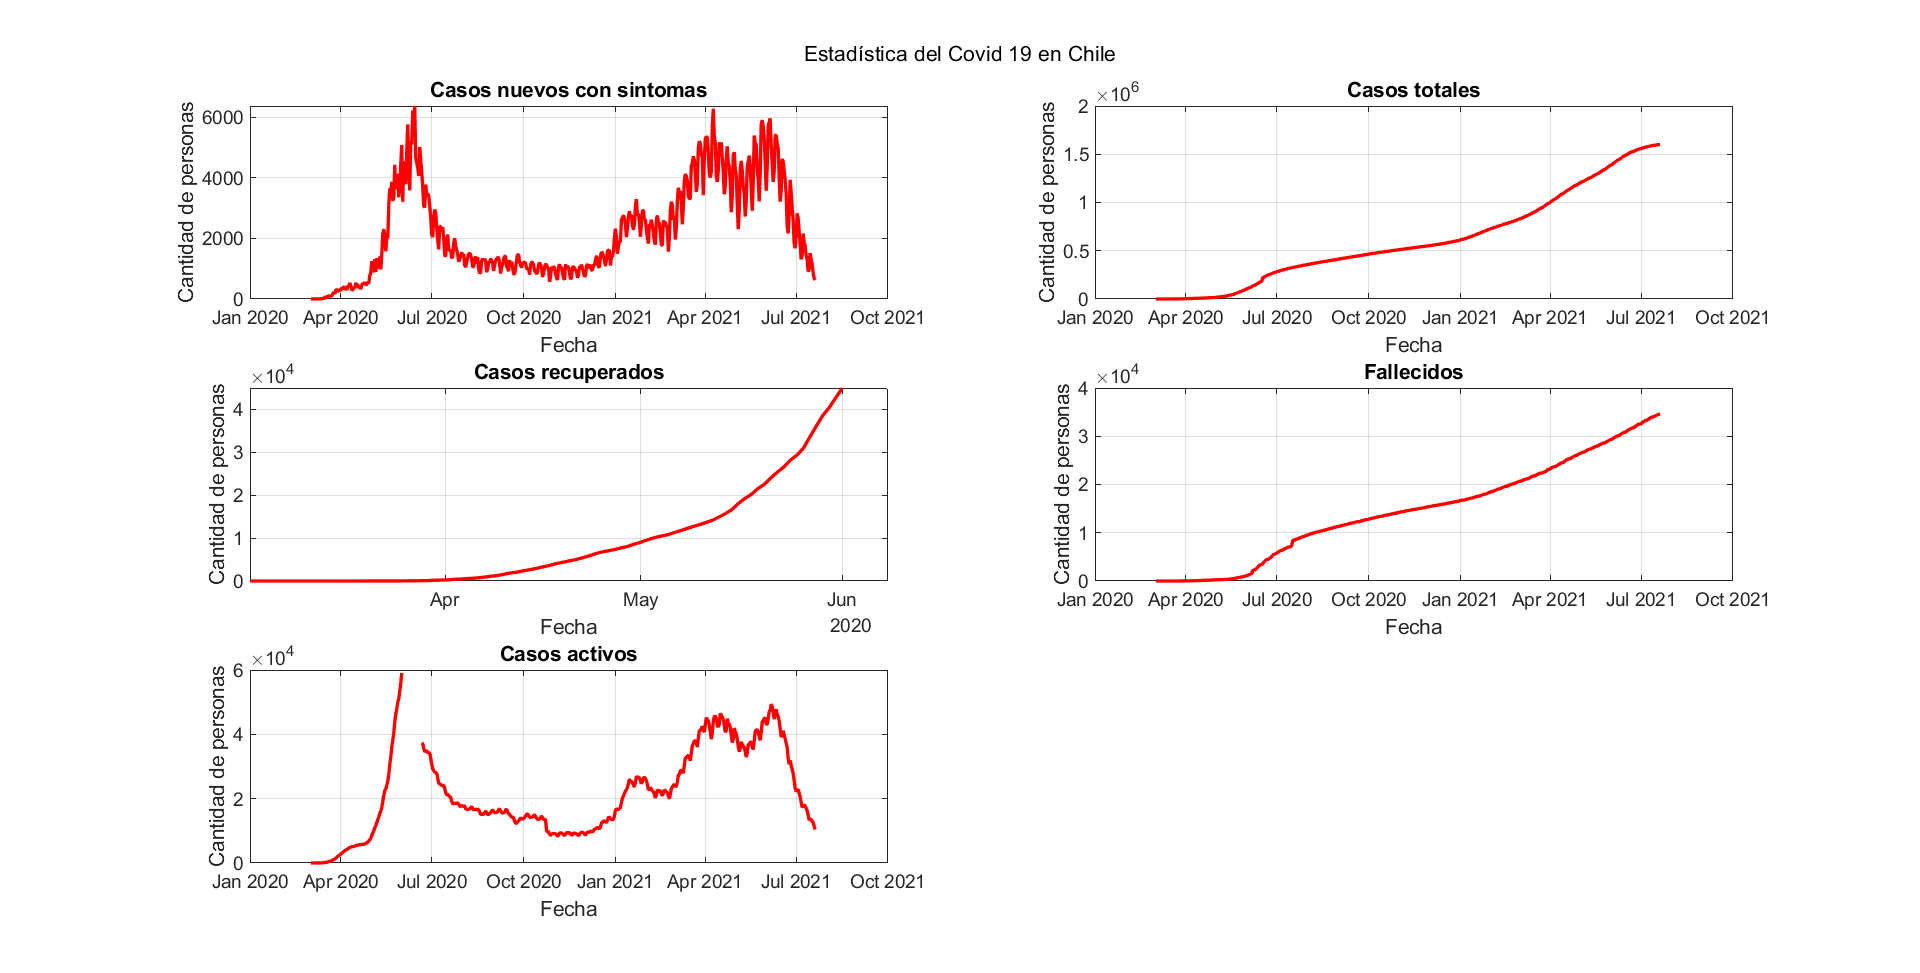
\includegraphics[width=1.1\textwidth]{Matlab/covidstat}
	\caption{Estadísticas del Covid19 en Chile}
	\label{fig:covidstat}
\end{figure}
\newpage

\subsection{Ejercicio 2}

A partir de la siguiente pagina web:\\
\url{https://mawun.cr2.cl/}\\
Descargue los datos de precipitación de la estación pluviométrica más cercana a donde vive.
Manipule los datos para que se puedan leer en Matlab y haga un gráfico que muestre los datos y el promedio de los días en que \textbf{SI} hubo precipitación(precipitación$>0$). Recuerde cambiar los -9999 por NaN.\par
\begin{figure}[h]
	\centering
	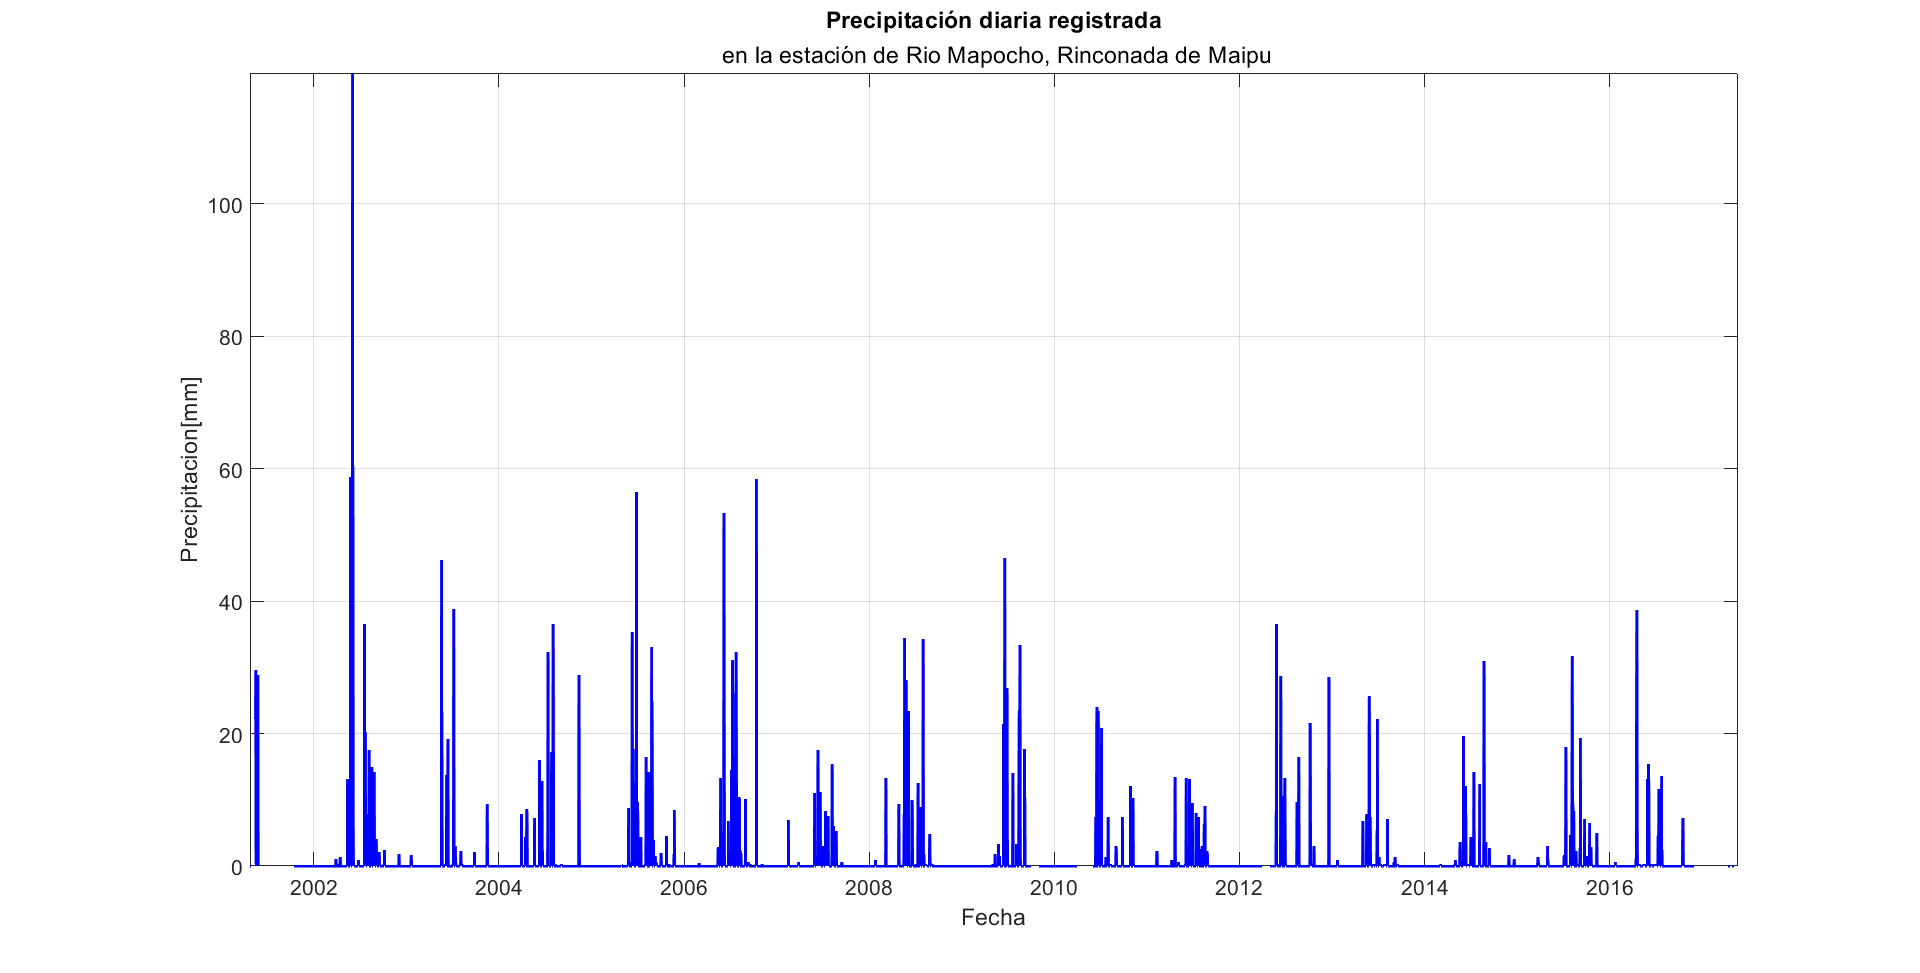
\includegraphics[width=1\linewidth]{Matlab/maipu}
	\caption{Precipitación diaria en Maipú}
	\label{fig:maipu}
\end{figure}
\newpage
\section{Guía 8}
\subsection{Ejercicio 1}
Genere una función que pida ingresar los datos y el número del ajuste(1 lineal,2 cuadratica,etc), y que genere una figura con los datos,el promedio, y su curva ajustada.Ejemplo: ajuste([1 9 2 5 3 4 6 7 8 1 9 4 8 5],3) genera la siguiente figura:\par
\begin{figure}[h]
	\centering
	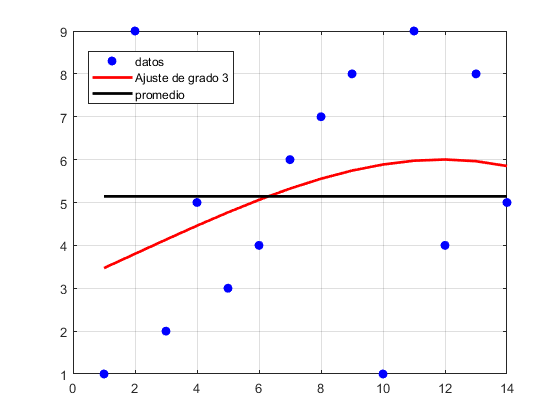
\includegraphics[width=1\linewidth]{Matlab/est1}
	\caption{}
	\label{fig:est1}
\end{figure}
\newpage
\subsection{Ejercicio 2}
Genere una función que al ingresar los datos y el rango, realice la media móvil de los datos, la desviación estándar móvil  y grafique ambas en una figura. ejemplo en la figura
\begin{figure}[h]
\centering
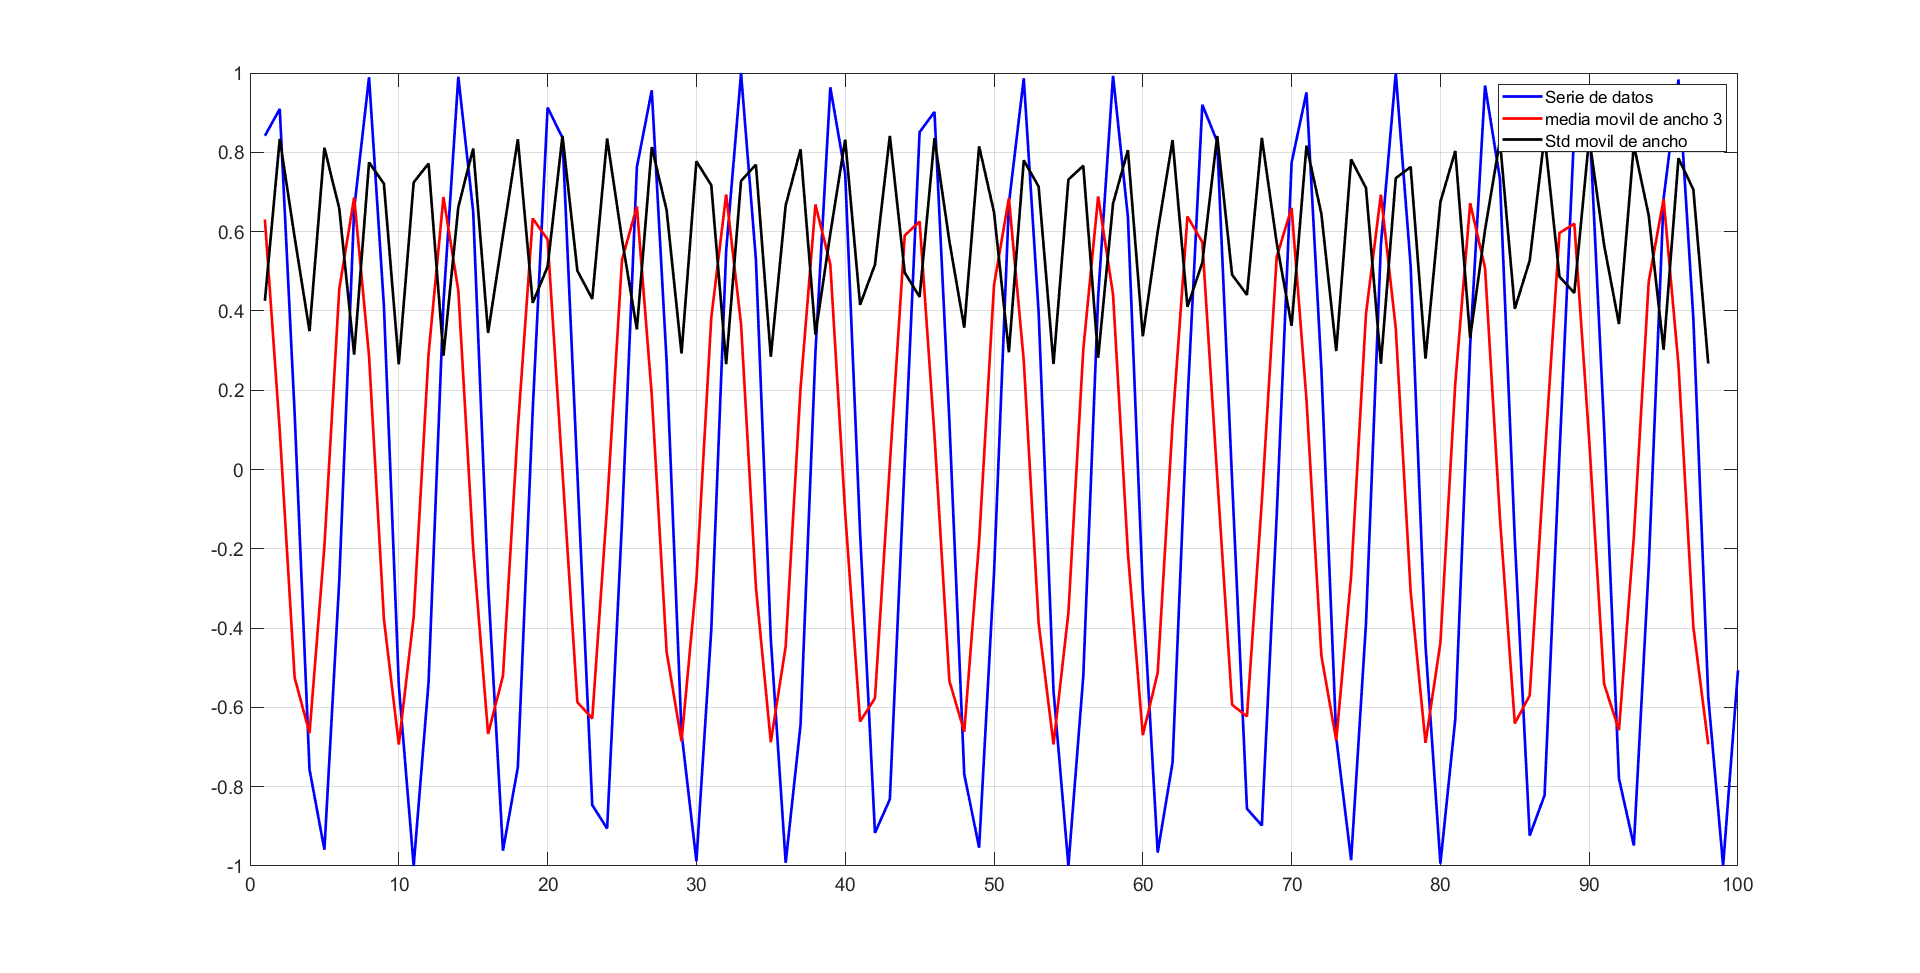
\includegraphics[width=1\linewidth]{Matlab/mmovil}
\label{fig:mmovil}
\end{figure}
\newpage
\section{Guía 9}
\subsection{Ejercicio 1}
Realice un mapa de la ruta mas corta entre la capital en donde vive, y dos lugares a donde usted quisiera viajar, como se ve en la figura(Capital inicial: Santiago, Destinos: Florida y Madrid):\par
\begin{figure}[h]
	\centering
	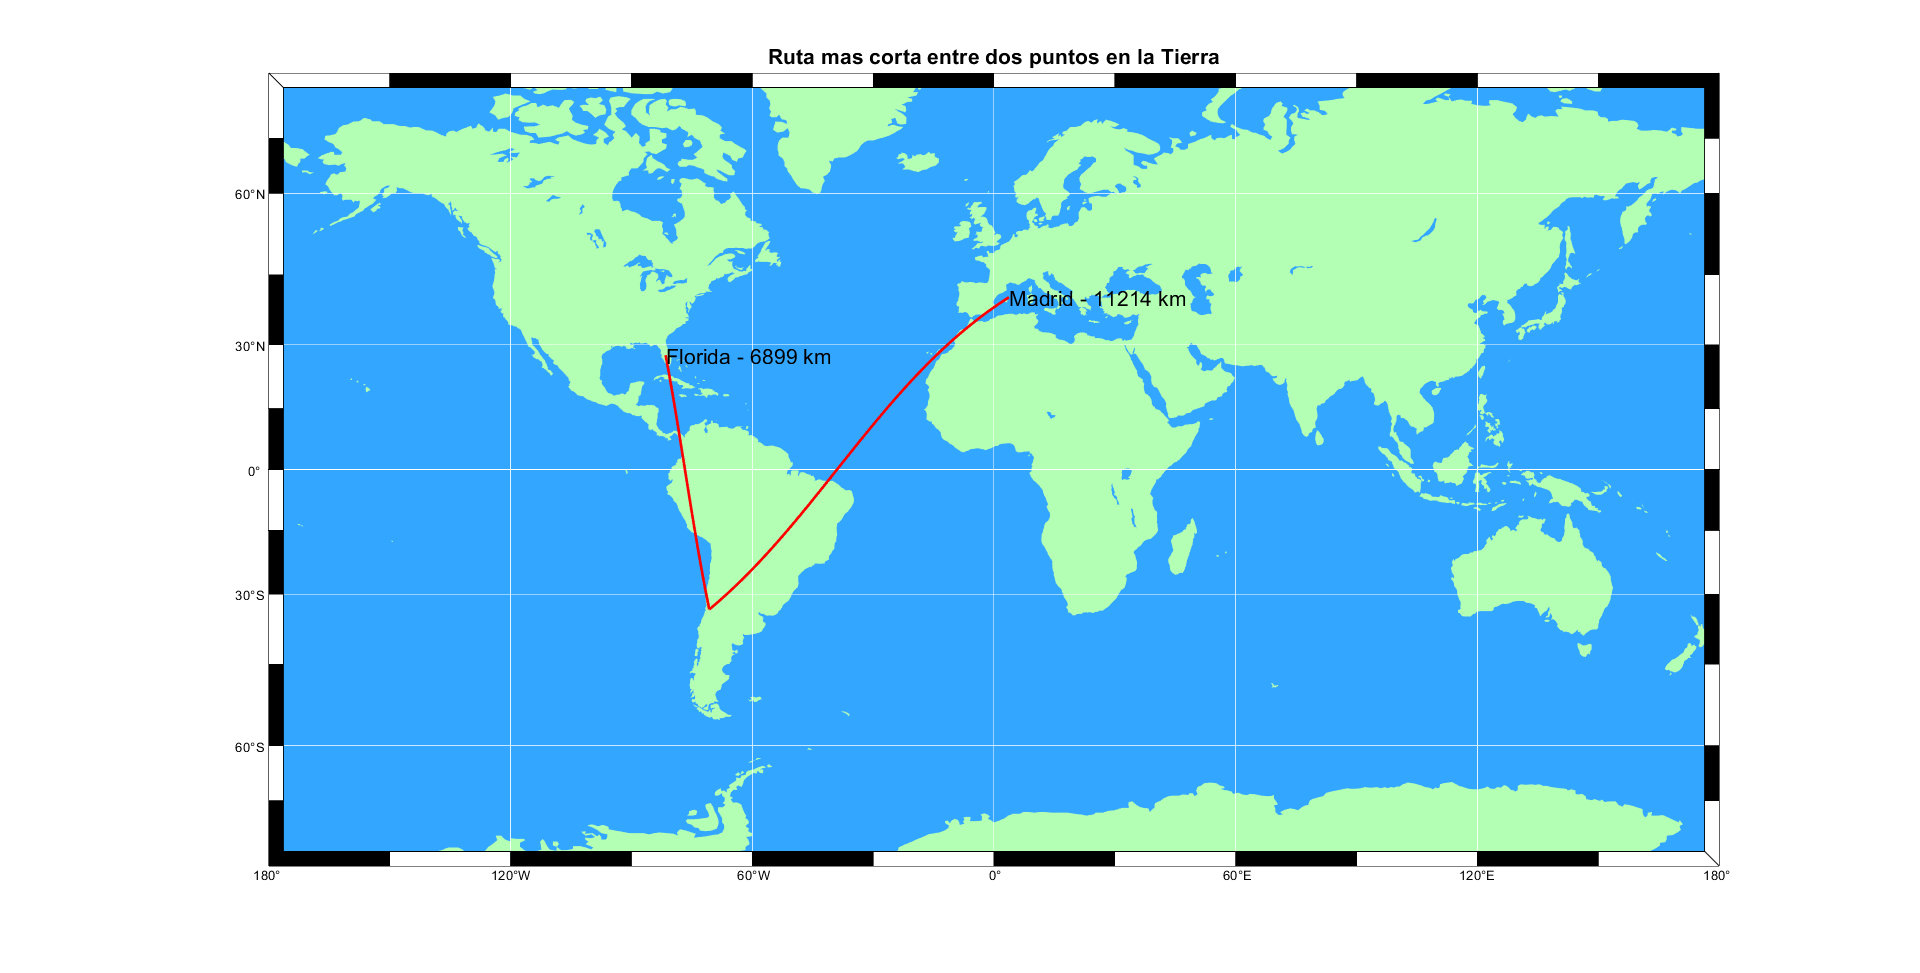
\includegraphics[width=1\linewidth]{Matlab/mapa1}
	\caption{Ruta mas corta entre dos puntos en la Tierra}
	\label{fig:mapa1}
\end{figure}
\newpage
\subsection{Ejercicio 2}
Realice un mapa de las condiciones meteorológicas como el de la figura pero en la fecha de su cumpleaños(dia y mes). Los archivos que necesita se encuentran en:\\
\url{https://github.com/alvillaca/Files-PNG/blob/main/Guia\%20Mapas/meteo.zip}
\begin{figure}[h]
	\centering
	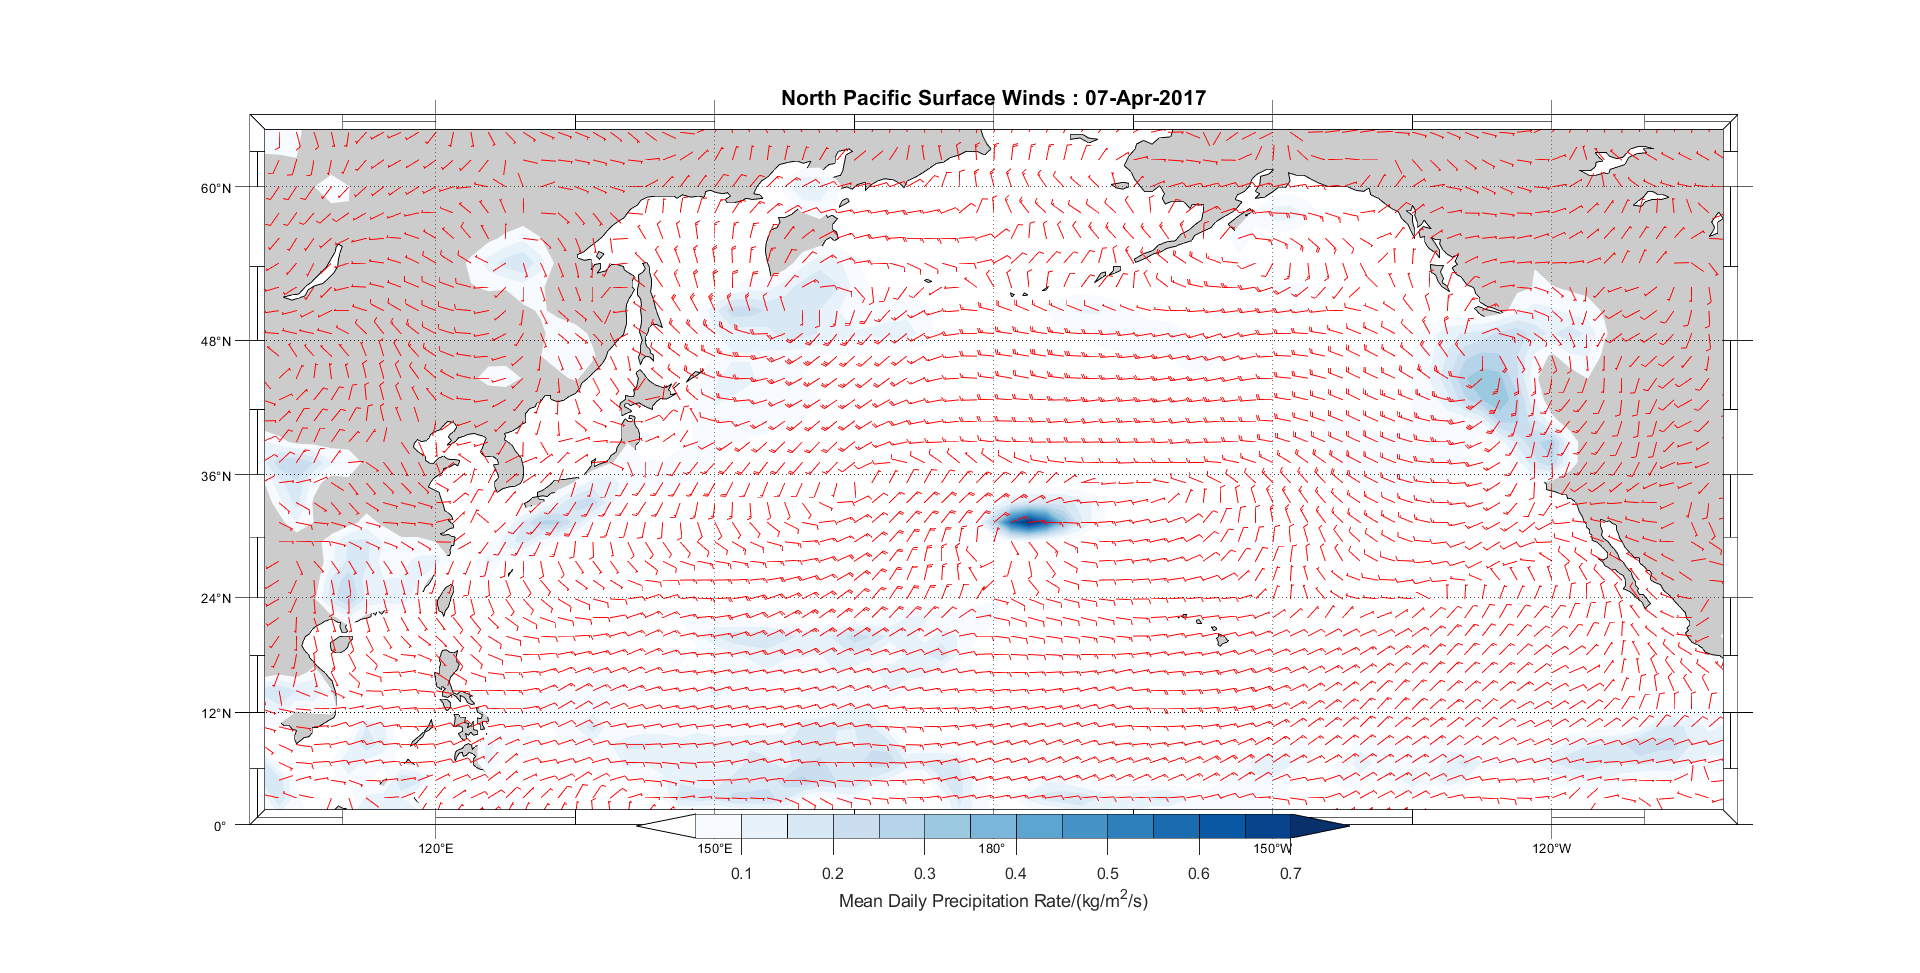
\includegraphics[width=1\textwidth]{Matlab/mapa}
	\label{fig:mapa}
\end{figure}
\newpage
\section{Guía 10}
\subsection{Ejercicio 1}
Grafique en Matlab el campo vectorial como se muestra en la figura:
\begin{equation}
	F(x,y)=\langle ln(1+y^{2}),ln(1+x^{2}) \rangle
\end{equation}.\par 
\begin{figure}[h]
	\centering
	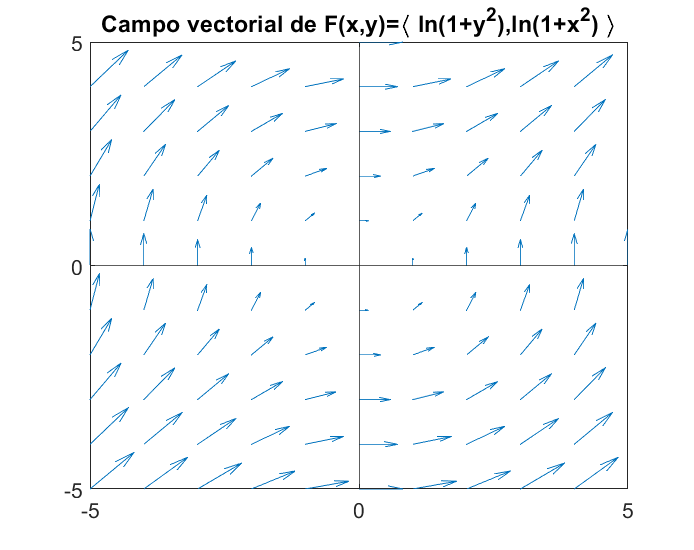
\includegraphics[width=0.7\linewidth]{Matlab/vectores}
	\label{fig:vectores}
\end{figure}\newpage
\subsection{Ejercicio 2}
Grafique en Matlab el campo vectorial  tal como se muestra en la figura(recuerde agregar la caja que encierra al plot):
\begin{equation}
	F(x,y,z)= (y)i +(z)j+ (x)k
\end{equation}
\begin{figure}[h]
	\centering
	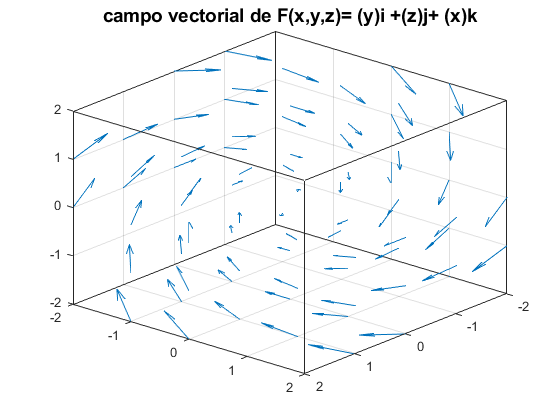
\includegraphics[width=0.7\linewidth]{Matlab/vec3d}
	\label{fig:vec3d}
\end{figure}
